\documentclass[]{llncs}
\usepackage{graphicx}

%\documentclass{article}
\usepackage{mathtools}



\usepackage{times}  % DO NOT CHANGE THIS
\usepackage{helvet} % DO NOT CHANGE THIS
\usepackage{courier}  % DO NOT CHANGE THIS
\usepackage[hyphens]{url}  % DO NOT CHANGE THIS
\usepackage{arydshln}
\usepackage{mathptmx}
\usepackage{amsmath}
\usepackage{bm}
\usepackage[english]{babel}
\usepackage[utf8]{inputenc}
\usepackage{algorithm}
\usepackage{epstopdf}
\usepackage{booktabs}
\usepackage{multirow}
\usepackage{siunitx}
\usepackage{rotating}
\usepackage{hyperref}
%\usepackage[algo2e]{algorithm2e}
%\usepackage{arevmath}     % For math symbols
\usepackage[noend]{algpseudocode}
\urlstyle{rm} % DO NOT CHANGE THIS
\def\UrlFont{\rm}  % DO NOT CHANGE T
% Used for displaying a sample figure. If possible, figure files should
% be included in EPS format.
%
% If you use the hyperref package, please uncomment the following line
% to display URLs in blue roman font according to Springer's eBook style:
% \renewcommand\UrlFont{\color{blue}\rmfamily}

\pagestyle{plain}
\setcounter{page}{1}
\pagenumbering{arabic}

\begin{document}

\title{Mathematics for Beliefs Strategy Approach}

\author{Frances Cameron-Muller, Supervisor: Dr. Julian Garcia}

\institute{Monash University}

\maketitle    

\section{Introduction}
In the beliefs strategy approach, each agent has an in and outgroup belief. These beliefs represent the probability of ingroup/outgroup individuals cooperating. 

\section{Definitions}
 
Payoff Matrix:
\begin{equation}
   \begin{pmatrix} 
   R & S  \\
   T & P  
   \end{pmatrix} 
\end{equation}

Payoff Threshold: $H = \frac{S-P}{T-P-R+S}$ \\
Focal player's ingroup belief:  $f_i$ \\  
Focal player's outgroup belief:  $f_o$ \\
Opponent player's ingroup belief:  $o_i$ \\ 
Opponent player's outgroup belief:  $o_o$ \\
Number of agents: $n$ \\ 
Proportion of tag 0s: $p$ \\ 
Number of rounds per step: $r$ \\ 

\section{Payoff of focal player of tag g against opponent player of tag t}

\[
   P_{g,t} =  \begin{cases}
        R & if\ f_t \geq H \cap o_g \geq H \\
        S & if\ f_t \geq H \cap o_g < H \\
        T & if\ f_t < H \cap o_g \geq H \\
        P & if\ f_t < H \cap o_g < H \\
    \end{cases}
\]

Let's introduce some indicator functions to represent the strategy a player $p$ will play against a tag group $t$ 
\[
   S_{p,t} =  \begin{cases}
        0 & if\ p_t \geq H \\
        1 & if\ p_t < H \\
    \end{cases}
\]

If a player's belief is above the threshold they will play a strategy of 0 (cooperation). 
In this case we are interested in the strategy if the focal player $f$ against the tag group of their opponent $t$ and vice versa.
\[
   S_{f,t} =  \begin{cases}
        0 & if\ f_t \geq H \\
        1 & if\ f_t < H  \\
    \end{cases}
\]
\[
   S_{o,g} =  \begin{cases}
        0 & if\ o_g\geq H \\
        1 & if\ o_g < H  \\
    \end{cases}
\]
\\
Therefore, \\
$P_{g,t} = R \times ( \, 1-S_{f,t}) \,  \times ( \, 1-S_{o,g}) \, + \ S \times ( \, 1- S_{f,t}) \, \times S_{o,g} \ + \ T \times S_{f,t} \times ( \, 1-S_{o,g}) \,\ + \ P \times S_{f,t} \times S_{f,t} $
\\
\\
Therefore, if you were given as input, g = tag group of the focal player, t = tag group of opposition, the in and outgroup beliefs of the focal and opponent player and the payoff matrix you can calculate the payoff of the focal player. 

This can be generalised to if you were given the average in and outgroup beliefs of the tag groups these can be used to approximate the beliefs for either or both players. 

Next, if we know the proportion of groups in the population, we can compute the expected payoffs and population payoffs. 
\\

Expected payoff per round for an agent of tag g $ = r \times p \times P_{g,o} \ + \ r\times(\, 1 - p )\, \times P_{g,1} $

\section{Graph} 
\begin{figure}
\centering
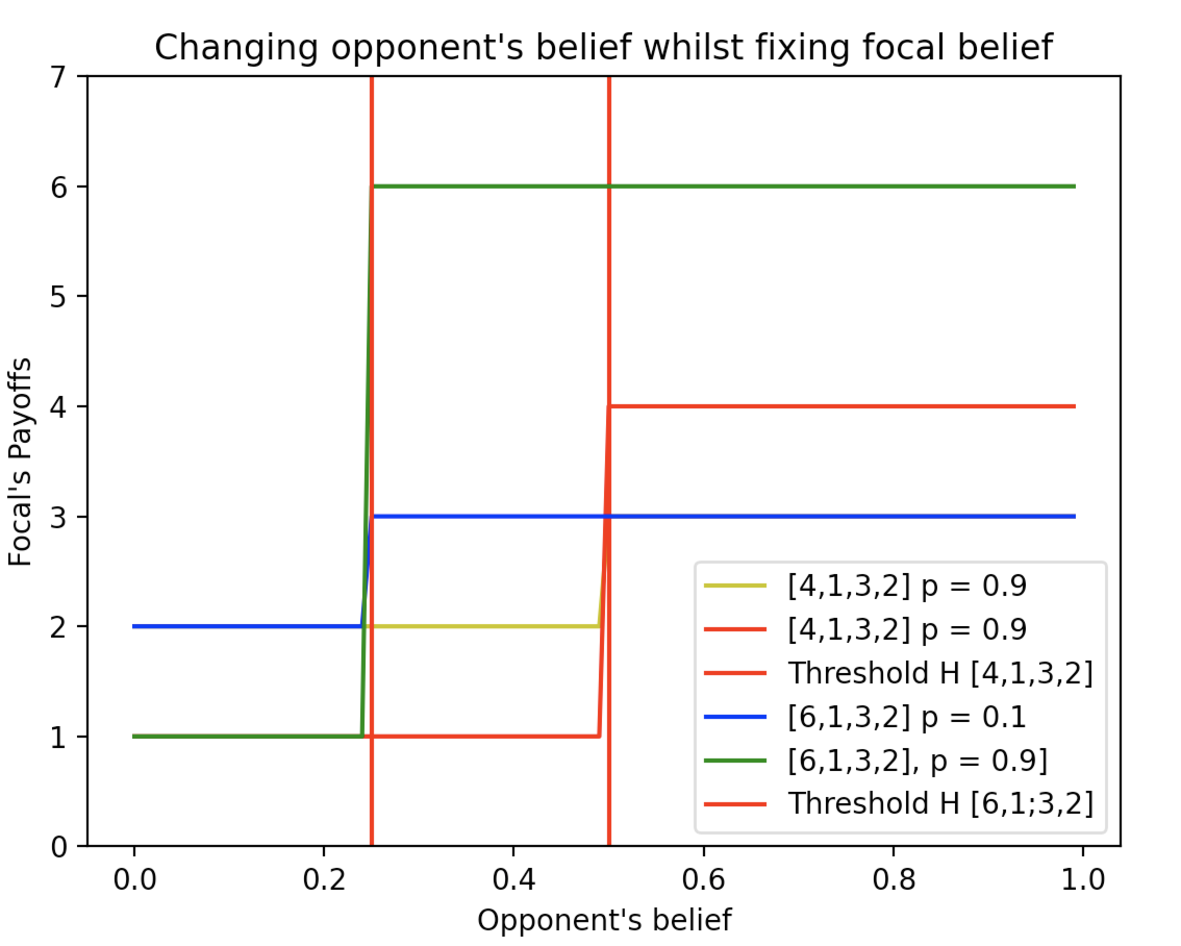
\includegraphics[width=15cm]{images/beliefs}
\caption{\label{beliefs} Graph of payoffs changing with beliefs.}
\end{figure}


\end{document}
